\addaj{
\vspace{-0.1in}
\section*{Appendix I - Will sampling be effective in the presence of very large skew?}
%\section{Appendix}
\label{sec:appendixSkew}
The task runtimes within a job may vary (\emph{skew}).  Intuitively, if the
skew across task sizes is small, sampling even a small number of pilot tasks
will be sufficient to yield an accurate estimate.

Our experiments using two different production cluster traces, which have
different types of job task size distribution, indicate that sampling is highly
effective for varying traces. Our rich trace analysis has shown that variation
in task size is not very high (\S\ref{sec:accuracy:trace}) and the job
execution settings (same code, same flags \etc) supports this
\cite{googleClusterData2011-2Schema, personalCommunication:MarkAstley}.
Additionaly, previous works like LATE~\cite{late:osdi08} and
SkewReduce~\cite{skewReduce:socc2010} have established mechanisms which will
prevent skew in task runtimes from high inflation.

We, however, believe that even if the skew across task sizes is very large as compared to the variation
across history sampling will not perform worse than history. 
%In the following, we give the intuition underpinning for why sampling will be
%effective even with very high skew.
In the following, we give both the intuition and quantitative underpinning for
why sampling is effective.

Consider, for example, two jobs and the simple setting where both jobs have
equal number of tasks. In order to improve the average JCT, we wish to schedule
the shorter job ahead of the longer job. If the total sizes of the two jobs are
very different, then even a moderate amount of estimation error of the job
runtimes will not alter their ordering. On the other hand, if the total sizes
of the two jobs are close to each other, then indeed the estimation errors will
likely alter their ordering. However, in this case since their sizes are not
very different anyway, switching the order of these two coflows will not
significantly affect the average JCT.

We quantitatively performed two simulations of job execution according to the
model defined in \S\ref{sec:accuracy:quantity} where we took $\sigmaonesqrd =
10000*\sigmanotsqrd$. In one simulation we kept difference between size of
$j_1$ and $\mu$ very large, $size(j_1) = 0.1\times \mu$, and in other we kept
them to be similar, $size(j_1) = 0.9\times \mu$. In each simulations we
considered 1000 jobs.  Figure~\ref{fig:numerical_analysis:highSkew} shows cdf
of individual JCT speedups. It can be seen that even with 10,000 time higher
variance across tasks, sampling is performing similar to history. This confirms
our intuition.

\begin{figure}[tp]
\centering
	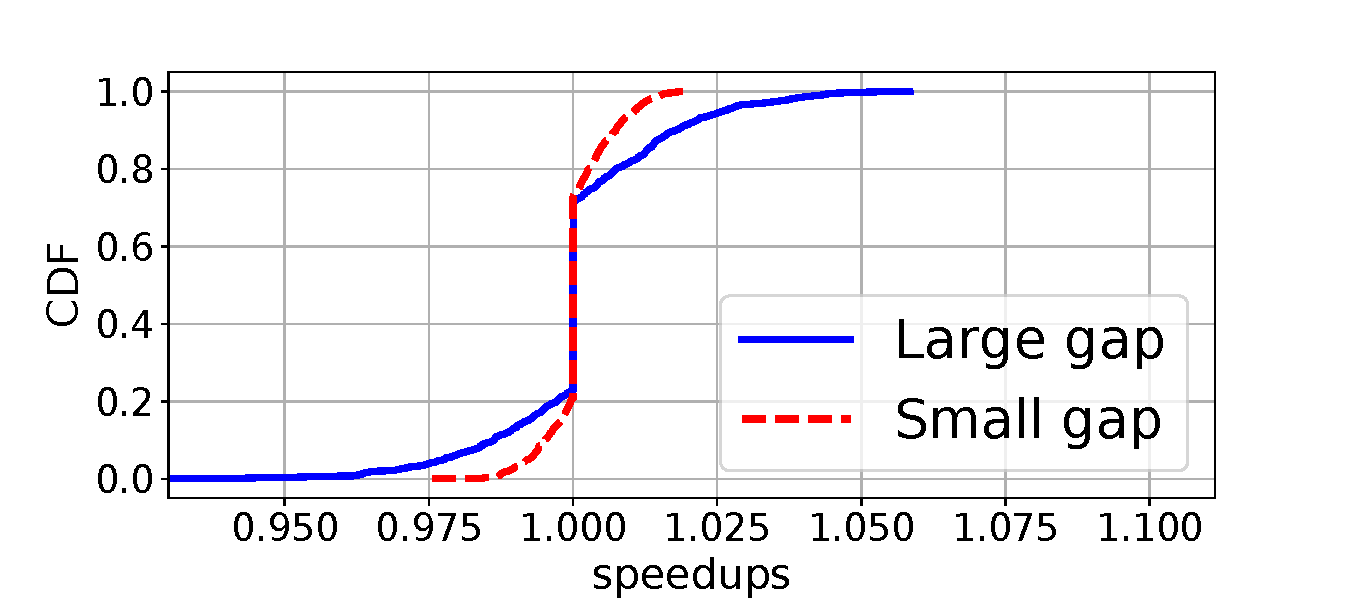
\includegraphics[width=1.0\linewidth]{figures/numerical_analysis/numerical_analysis_high_skew_speedup.pdf}
	\vspace{-0.1in}
\caption{Simulation results for job execution with very high task size skew.}
\label{fig:numericalAnalysis:highSkew}
\vspace{-0.2in}
\end{figure}


}
